%! Tex program = xelatex
\documentclass[UTF8]{article}
\usepackage{indentfirst}
\usepackage{graphicx} 
\usepackage{amsmath}  
\usepackage{float}   
\usepackage{listings}

\title{Discrete Mathematics}
\author{Zhengren Wang 2019081308021}
\date{06/02/2020 Tue}
\begin{document}
\maketitle 

\part{10.5}
\begin{description}
    \item[5]Determine whether the given graph has an Euler circuit. Construct such a circuit when one exists. If no Euler circuit exists, determine whether the graph has an Euler path and construct such a path if one exists.  \\
        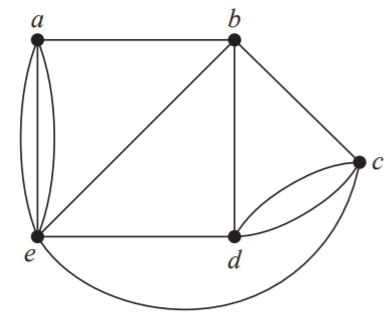
\includegraphics[scale=0.3]{../imgs/10_5_5.png}\\\\
            Euler circuit: $a, b, c, d, c, e, d, b, e, a, e, a$\\


    \item[39]Does the below graph have a Hamilton path? If so, find such a path. If it does not, give an argument to show why no such path exists.   \\
        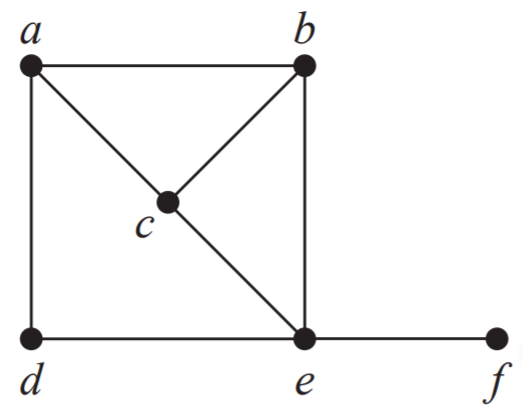
\includegraphics[scale=0.3]{../imgs/10_5_39.png}\\\\
            Hamilton path: $f, e, d, a, b, c$\\

\end{description}

\end{document}
